\section{Query Oriented Visual Tasks}
\label{sec-reinforcement-learning}
In this section, we introduce how we do visual tasks that are in connection with questions. 


\subsection{Visual Processing}
\label{sec-visual-processing}
\begin{figure}[h]
\begin{center}
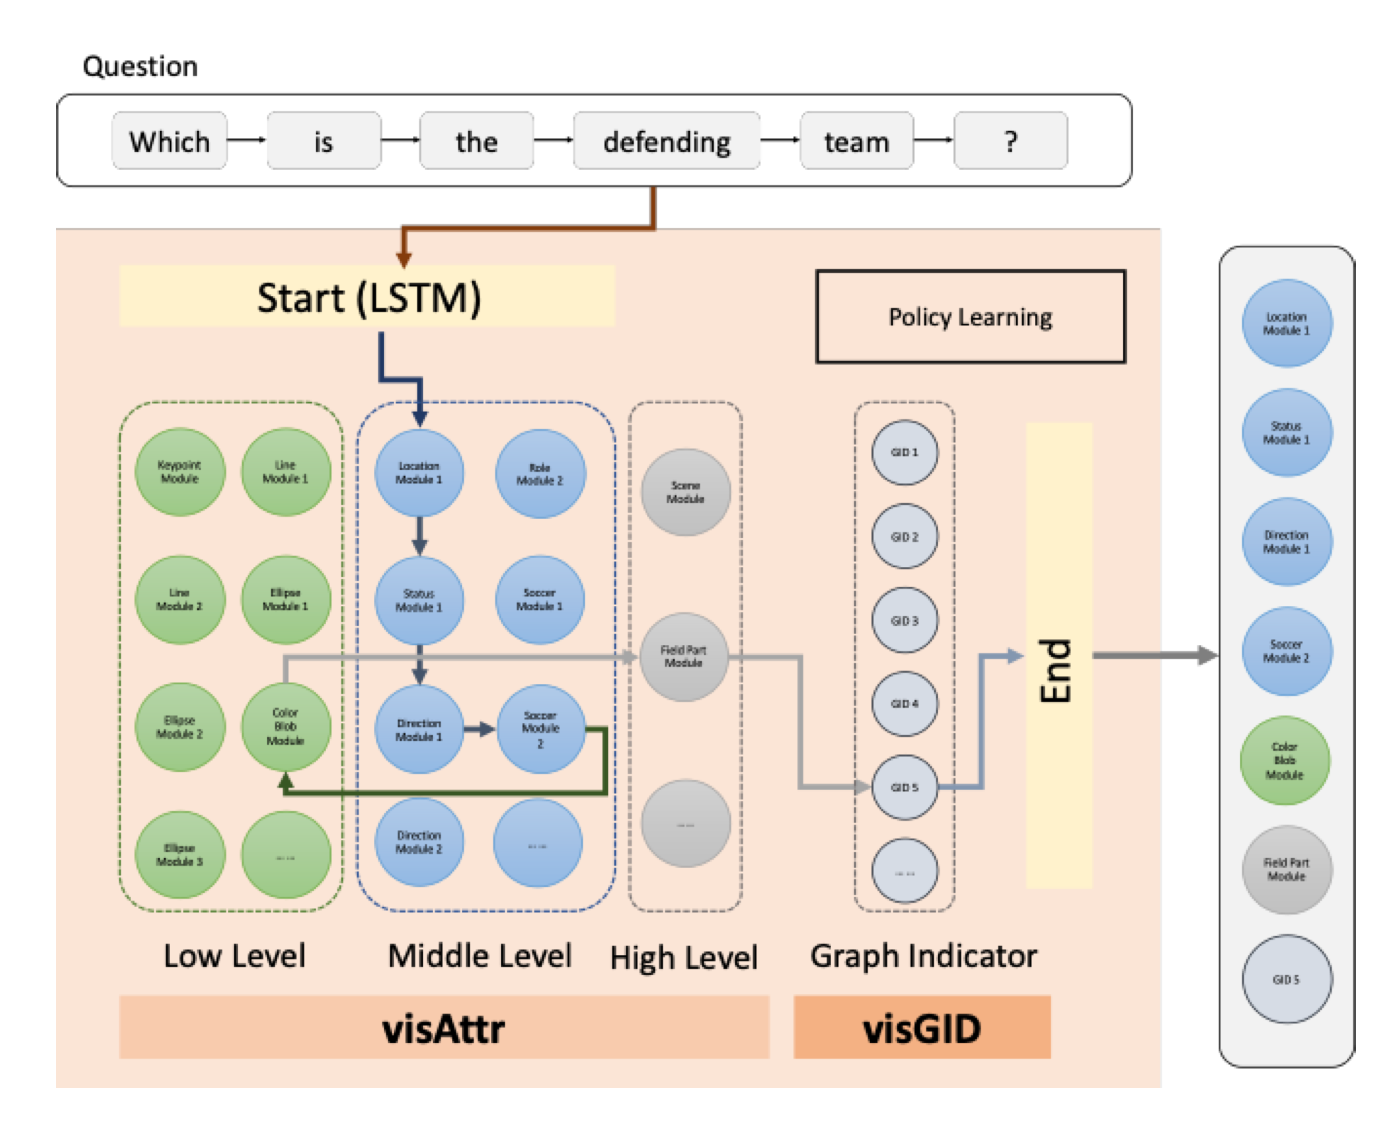
\includegraphics[width=\linewidth]{figure/RLplot.png}
\end{center}
\caption{Overview of our approach}
\label{fig:RLplot}
\end{figure}

In our approach, we build a structure which selects sub-tasks to form a policy which is based on queries. For instance, with the input \textit{which is the defending team?}, the system first predicts the corresponding steps are \textit{Human Module}, \textit{Gesture Module}, \textit{Direction Module}, \textit{Soccer Module}, \textit{Color Blob Module}, \textit{Field Part Module} and \textit{Graph Indicator}. Guided by such action sequence, the image features are extracted by operating relevant vision tasks. An overview is shown in Figure~\ref{fig:RLplot}.

\subsection{Visual Processing}
\label{sec-visual-processing}

\stitle{Multi-layer LSTM with Attention}\\
The task here is to predict the most suitable action module sequence by given questions and performance

We would like to predict the most suitable reasoning
structure tailored to each question. For an input question q
such as What object is next to the t
Figure~\ref{fig:Attention}





\stitle{Visual Task Pool}\\
First, the question features $w_{q,d}$ are extracted from questions by a Long short-term memory (LSTM) and comes into the step of visual task selection (\kw{VTS}). \kw{VTS} is guided by the question feature, selecting target visual tasks from the task pool by Monte Carlo learning. The task pool is demonstrated in Table~\ref{table:visual_tasks}.



% Please add the following required packages to your document preamble:
% \usepackage{multirow}
\begin{table}[]
\centering \scriptsize
\begin{tabular}{|l|ll|l|}
\hline
visAttr & \multicolumn{1}{l|}{Level}  & Sub-task           & Descriptions                                                                                                                                 \\ \cline{2-4} 
        & \multicolumn{1}{l|}{Low}    & Keypoint Module    & \multirow{3}{*}{\begin{tabular}[c]{@{}l@{}}To get detailed information of the \\ soccer field. $F_{keypoint}$\end{tabular}}                  \\ \cline{3-3}
        & \multicolumn{1}{l|}{}       & Line Module        &                                                                                                                                              \\ \cline{3-3}
        & \multicolumn{1}{l|}{}       & Ellipse Module     &                                                                                                                                              \\ \cline{3-4} 
        & \multicolumn{1}{l|}{}       & Color Blob Module  & \begin{tabular}[c]{@{}l@{}}To detect blobs of different color \\ among a region(whole soccer \\ field or a small bounding box).\end{tabular} \\ \cline{2-4} 
        & \multicolumn{1}{l|}{Middle} & Location Module    & \begin{tabular}[c]{@{}l@{}}To detect the location of the \\ person. $P_{location}$\end{tabular}                                              \\ \cline{3-4} 
        & \multicolumn{1}{l|}{}       & Status Module      & \begin{tabular}[c]{@{}l@{}}To get the person's gesture \\ $P_{status}$ (standing, moving, \\ expansion).\end{tabular}                        \\ \cline{3-4} 
        & \multicolumn{1}{l|}{}       & Direction Module   & \begin{tabular}[c]{@{}l@{}}To get whether a person is facing\\ the goal or not.\\ $P_{direction}$\end{tabular}                               \\ \cline{3-4} 
        & \multicolumn{1}{l|}{}       & Uniform Module     & \begin{tabular}[c]{@{}l@{}}To get the uniform color of the \\ person $P_{uniform}$\end{tabular}                                              \\ \cline{3-4} 
        & \multicolumn{1}{l|}{}       & Soccer Module      & \begin{tabular}[c]{@{}l@{}}To detect the location of the \\ soccer. $S_{location}$\end{tabular}                                              \\ \cline{2-4} 
        & \multicolumn{1}{l|}{High}   & Field Part Module  & \begin{tabular}[c]{@{}l@{}}To detect which part of the\\ soccer field is there in the \\ image $F_{part}$ .\end{tabular}                     \\ \hline
visGID  &                             & Graph ID Indicator & \begin{tabular}[c]{@{}l@{}}To indicate which type of graph\\ will be used in \\ the following process.\end{tabular}                          \\ \hline
\end{tabular}
\caption{Visual Task Pool}
\label{table:visual_tasks}
\end{table}



The pool is constructed by two parts, the first one is \textit{visAttr} which aims to discover the attribute of people, soccer, field and scene~\cite{peixi2019}, while the other one \textit{visGId} is an indicator showing the current question belongs to which graph type. There are three levels of \textit{visAttr}: low, middle and high, which represents different difficulty degree of the vision tasks. 

For each vision task, the approach is not fixed, one task can be achieved by different methods with variance in time and accuracy. For instance, object detection based methods, like Faster R-CNN~\cite{Ren:2015:FRT:2969239.2969250}, R-FCN~\cite{DBLP:conf/nips/DaiLHS16}, SSD~\cite{DBLP:conf/eccv/LiuAESRFB16} or skeleton keypoints detection based method like~\cite{cao2017realtime} and~\cite{wei2016cpm} can be implemented as a set of status module methods, because all of them is able to localize and distinguish people who are moving, standing or with an expansion gesture (Figure~\ref{fig:Person Status}). 

\begin{figure}[thb]
\centering
        \begin{subfigure}[b]{0.088\textwidth}
                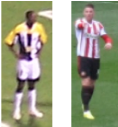
\includegraphics[width=\linewidth]{figure/stand1.png}
                \caption{Standing}
                \label{fig:gull}
        \end{subfigure}\quad
        \begin{subfigure}[b]{0.127\textwidth}
                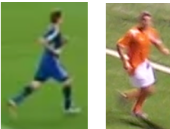
\includegraphics[width=\linewidth]{figure/move1.png}
                \caption{Moving}
                \label{fig:gull2}
        \end{subfigure}\quad
        \begin{subfigure}[b]{0.166\textwidth}
                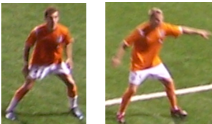
\includegraphics[width=\linewidth]{figure/expand1.png}
                \caption{Expansion}
                \label{fig:tiger}
        \end{subfigure}
        \caption{Person status.}\label{fig:Person Status}
\end{figure}




\begin{figure}[h]
\begin{center}
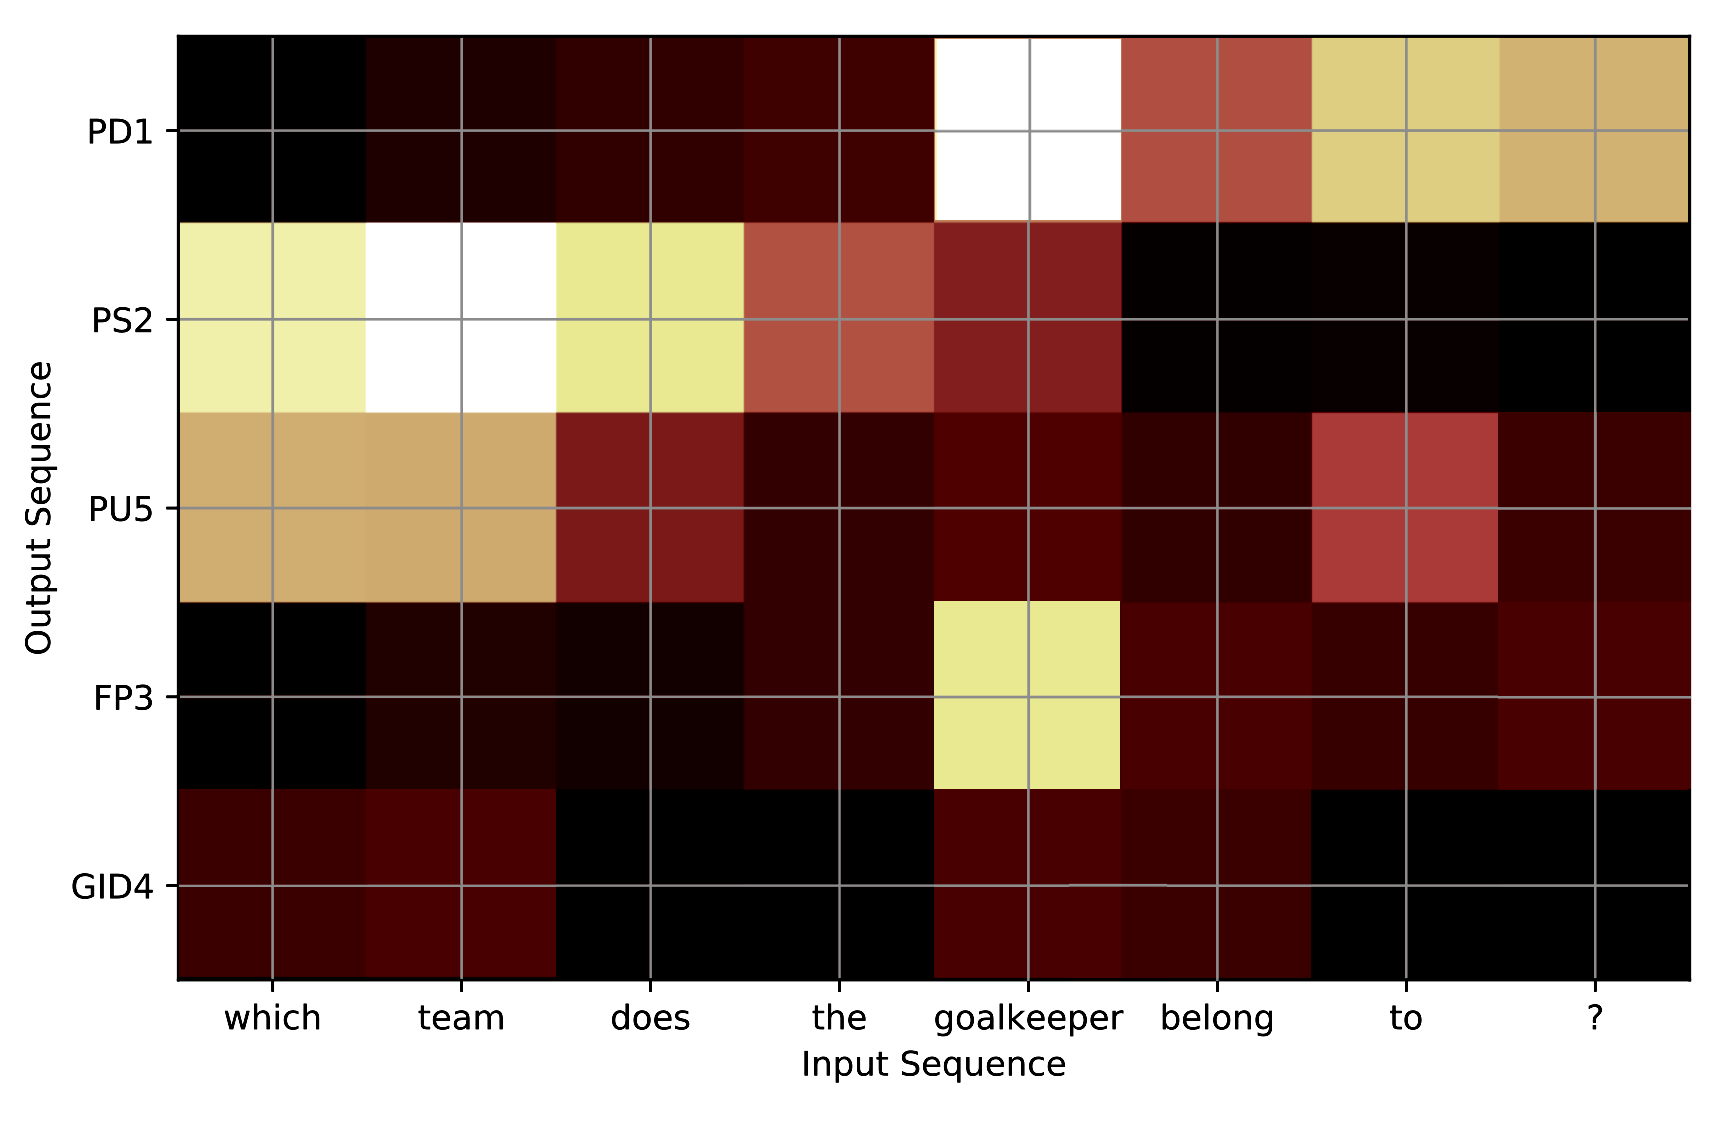
\includegraphics[width=\linewidth]{figure/question.png}
\end{center}
\caption{Attention Mechanism in Query}
\label{fig:Attention}
\end{figure}


\stitle{Time and Accuracy Term}\\
VQA is a topic in real-time domain, which leads that the answering time cannot be directly ignored, meanwhile, the accuracy still plays a significant role. To better balance these two, we proposed time and accuracy terms in loss function of training process.

\stitle{Monte Carlo Methods}

\subsection{Construction of \kw{EAG}}
\label{sec-eag-construction}

After objects that are related to questions are identified, we construct a graph structure, denoted as \kw{EAG}, along the same line as~\cite{peixi2019}. 


\begin{example}
\label{exm-x1}
ADD AN EXAMPLE TO ILLUSTRATE PROGRESS IF NECESSARY!
\end{example}
